\documentclass[a4paper,preprint]{sig-alternate}

\usepackage{times}
\usepackage{helvet}
\usepackage{courier}
\usepackage{microtype}
\usepackage{hyperref}

\frenchspacing

\toappear{}

\usepackage{blindtext}

\begin{document}

\title{Robustness \& Graph (Convolutional) Neural Networks}

\numberofauthors{1}
%
\author{
%
\alignauthor Tim Bohne\\
\email{tbohne@uni-osnabrueck.de}
}

\maketitle

% TODO: Gliederung für das Paper überlegen / Referenzen / stichpunktartig Inhalte andeuten

\begin{abstract}
\begin{quote}
TBD
\end{quote}
\end{abstract}

\section{Introduction}

The intent of this paper is to provide a concise overview of the current state of research in the domain of graph (convolutional) neural networks
with a focus on the robustness of these models. Since they have proven to be quite successful in various practical applications, 
it is quite obvious that the robustness of such models is of relevance.
After presenting some motivation and background for graph neural networks (GNNs) and particularly graph convolutional networks (GCNs)
and their possible practical applications in section \ref{sec:background}, an overview of the current state of the literature is
provided in section \ref{sec:literature}. Subsequently, the core ideas, methods, and results of the first works on certifiable
robustness of GNNs are introduced in section \ref{sec:main_section}.
Finally, there is a conclusion and a brief outlook on possible future research in section \ref{sec:conclusion}.

\section{Background}
\label{sec:background}

A currently very active research area inside the field of machine learning or more precisely deep learning considers models to learn
from graph inputs. Those models are called graph neural networks (GNNs). Graphs are useful data structures in complex real-life
applications such as modeling physical systems, learning molecular fingerprints, controlling traffic networks, and recommending 
friends in social networks.\cite{article}
Therefore, it is reasonable to think about combining graphs as data structures with state-of-the-art machine learning models.
However, these tasks require dealing with non-Euclidean graph data that contains rich relational information between elements and
cannot be well handled by traditional deep learning models which usually work with data represented in the Euclidean domain, e.g. in the
fields of computer vision (images) or natural language processing (text).\cite{article}
There are numerous reports of convincing performance of GNNs in practical applications (e.g. (add sources)),
especially in the task of semi-supervised node classification.\cite{xu2019topology}
Further typical applications for graphs as non-Euclidean data structure in machine learning are link prediction and clustering.\cite{zhou2019graph}
In summary, GNNs are models to conduct deep learning with graph data.

\subsection{Motivation}

One of the most successful type of model in the field of deep learning is the convolutional neural network (CNN).
GNNs are motivated by CNNs which are capable of extracting and composing multi-scale localized spatial features
for features of high representational power, but can only operate on Euclidean data like images and text.\cite{article}
Thus, the idea is to generalize CNNs to graphs.\newline
Another motivation comes from graph embedding, which learns to represent graph nodes, edges, or subgraphs in low-dimensional vectors.\cite{article}
The authors also highlight that traditional machine learning approaches for graph analysis rely on hand-engineered features which causes them
to be rather inflexible and expensive.

\subsection{Graph Neural Networks}

In this section, the basic graph neural network model proposed by Scarselli et al. \cite{4700287} gets introduced
based on the description in \textit{'Introduction to graph neural networks'}\cite{article}.\newline
The goal of a GNN is to learn a state embedding $h_v \in \mathbb{R}^S$ for each node that is used to produce an 
output $o_v$, e.g. the distribution of the predicted node label.
The original GNN model works with an undirected homogeneous graph where each node $v$ in the graph has its input features $x_v$
as well as a set of edges $co[v]$ and neighbors $ne[v]$. The authors illustrate the structure with the example in fig. \ref{fig:graph}
where $x_{1}$ is the input feature of $l_1$, $co[l_1]$ contains the edges $l_{(1, 4)}, l_{(1, 6)}, l_{(1, 2)}$, and $l_{(3, 1)}$ and $ne[l_1]$
contains nodes $l_2, l_3, l_4,$ and $l_6$.

\begin{figure}[h]
    \centering
    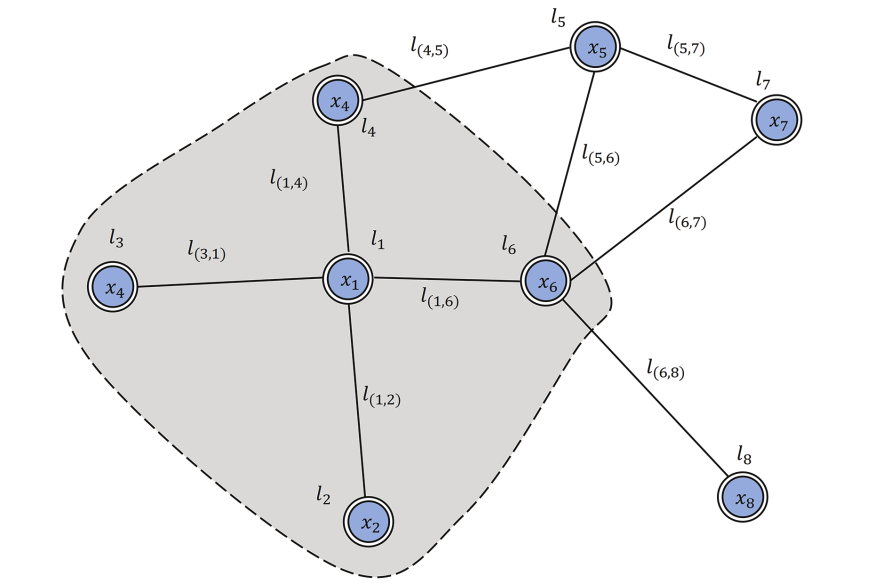
\includegraphics[width=0.4\textwidth]{img/graph.png}
    \caption{Example of the graph based on Scarselli et al. \cite{article}}
    \label{fig:graph}
\end{figure}

There are two important functions, $f$ updates the node state based on the input neighborhood and $g$ computes the output of a node.
Let $x$ be the input feature and $h$ the hidden state:
\begin{itemize}
    \item \textbf{node embedding:} $h_v = f(x_v, x_{co[v]}, h_{ne[v]}, x_{ne[v]})$
    \item \textbf{output embedding:} $o_v = g(h_v, x_v)$
\end{itemize}

Usually, $h_v$ and $o_v$ are described in a more compact form as matrices of stacked states,
outputs, and features with $F$ and $G$ being the stacked versions of $f$ and $g$:
\begin{itemize}
    \item $H = F(H, X)$
    \item $O = G(H, X_N)$
\end{itemize}

The $t$-th iteration of $H$ is described as $H^{t + 1} = F(H^t, X)$.
Using the target information $t_v$ for node $v$, the loss can be written as $\sum_{i=1}^p (t_i - o)$
where $p$ is the number of supervised nodes. The learning algorithm is based on a gradient-descent strategy.\newline

\vfill
\pagebreak

This basic GNN model provides a first step towards incorporating neural networks into the graph domain, 
but has several limitations \cite{article} which are tackled in various variants of GNNs such as graph convolutional networks (GCNs).

\subsection{Robustness}

Besides the repeatedly demonstrated good performance, there is one big issue which is subject to a rather new branch of 
research inside the field of GNNs which is the robustness of such models. There are several publications that analyze 
the robustness of GNNs to adversarial examples and recently there came up first approaches to strengthen
or even to certify their robustness with regard to a certain perturbation set.\newline
Recent advancements in deep neural networks for graph-structured data have led to state-of-the-art performance on recommender system benchmarks.\cite{Ying_2018}
The authors describe a large-scale deep recommendation engine that they developed and deployed at a major tech company.
This example illustrates the need for robust GNNs. Although these systems may be relatively rare in practical applications, especially at
that scale, at the moment, their performance suggests that they will be soon. However, in order to be able to use such models
with a clear conscience in practical applications requires a certain degree of robustness.
The vulnerability to adversarial attacks has raised increasing concerns for applying GNNs in safety-critical applications.\cite{jin2020graph}\newline

\textbf{Adversarial Perturbations}\newline

A well-studied problem of machine learning models in general is the sensitivity to adversarial perturbations.\cite{goodfellow2015explaining}
The idea of such perturbations, which is visualized in fig. \ref{fig:adversarial_example}, is that slight changes to the input data
cause an entirely different output of the model and therefore often misclassification.

\begin{figure}[h]
    \centering
    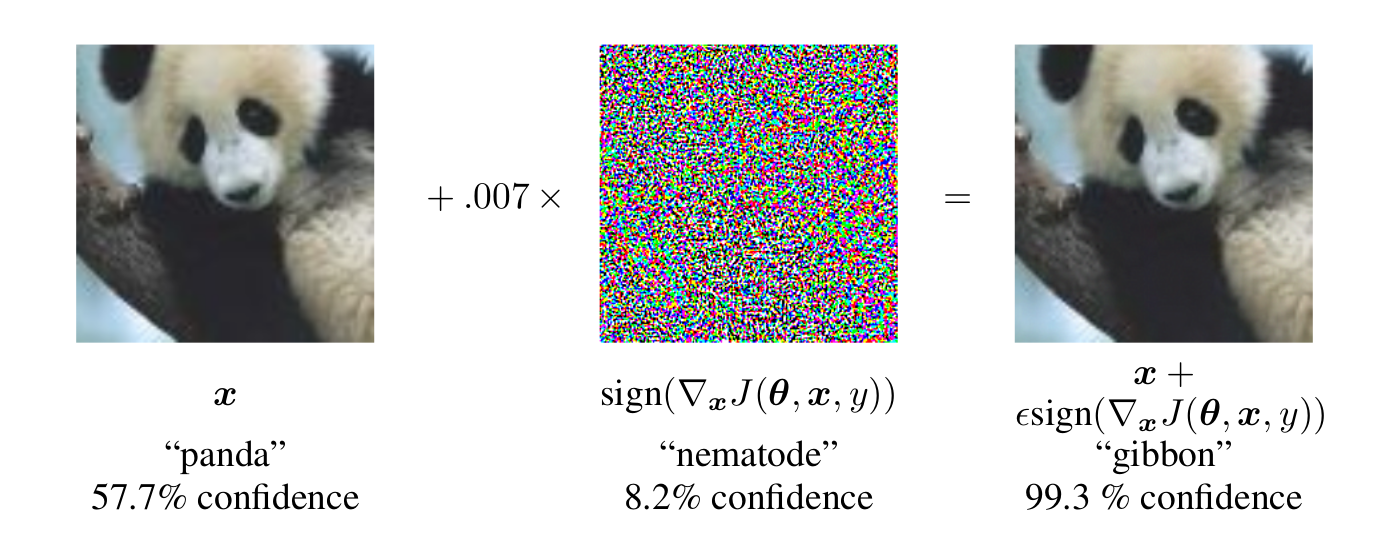
\includegraphics[width=0.5\textwidth]{img/adversarial_example.png}
    \caption{Demonstration of fast adversarial example. \cite{goodfellow2015explaining}}
    \label{fig:adversarial_example}
\end{figure}

Goodfellow et al. \cite{goodfellow2015explaining} face that problem by adversarial training which means that they include adversarially 
perturbed examples into the training procedure to strengthen the robustness of the models. They also introduce fast methods for generating 
those adversarial examples such as displayed in fig. \ref{fig:adversarial_example}. By adding an imperceptibly small vector whose elements
are equal to the sign of the elements of the gradient of the cost function with respect to the input, they can change GoogleNet's classification
of the image.\cite{goodfellow2015explaining}\newline
Adversarial perturbations are not only a problem for classical machine learning models, but also for GNNs.
Recent works show that graph neural networks are highly non-robust with respect to adversarial attacks on both the graph
structure and the node attributes, making their outcomes unreliable.\cite{Z_gner_2019}
Similarly to the example in fig. \ref{fig:adversarial_example}, small perturbations to the graph structure and node features lead to 
misclassification of the target as depicted in fig. \ref{fig:adversarial_GNN}.

\begin{figure}[h]
    \centering
    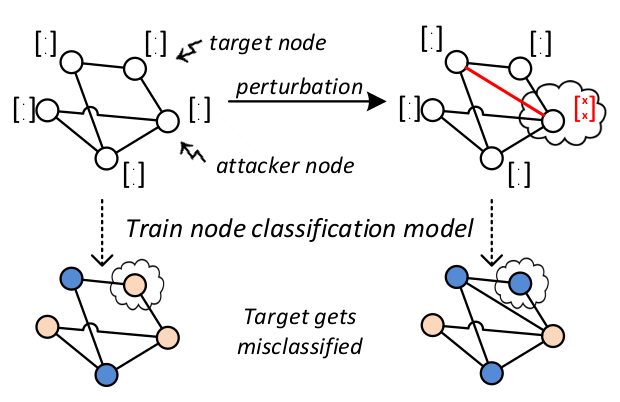
\includegraphics[width=0.35\textwidth]{img/adversarial_GNN.png}
    \caption{Small perturbations of the graph structure and node features lead to misclassification of the target. \cite{Z_gner_2018}}
    \label{fig:adversarial_GNN}
\end{figure}

\vfill
\pagebreak

\section{Literature Review}
\label{sec:literature}

This section will provide an overview of the current state of research in the domain of robust GNNs which could be divided
roughly into three important phases.
The first phase was to show that GNNs are indeed vulnerable to adversarial perturbations of the graph structure and the node attributes (cf. \ref{sec:rev1}).
Afterwards, in the second phase, several publications introduced defense mechanisms against such attacks or novel training procedures 
to strengthen the robustness of the models in some scenarios (cf. \ref{sec:rev2}). Only recently, the third phase began in which first approaches appeared
that are able to not only provide mitigations to adversarial attacks in some scenarios, but to give provable guarantees about the (non-)robustness 
of a model which is key to use them in safety-critical applications in the real world (cf. \ref{sec:rev3}). Because of the relevance of the last phase, which 
is an important step in the process of bringing the convincingly performing GNN models into the real world, the main focus of the following sections
will be on publications from that phase.

\subsection{Vulnerability of GNNs to adversarial perturbations}
\label{sec:rev1}

Dai et al. \cite{dai2018adversarial} focus on adversarial attacks on graph structured data that fool the model by modifying the
combinatorial structure of the data. They use synthetic and real-world data to show that a family of GNN models is vulnerable
to these attacks in both graph-level and node-level classification tasks.
Another approach for adversarial attacks on graph structured data is proposed by Zügner et al. \cite{Z_gner_2018} who focus on node classification
via graph convolutional networks.
The authors claim that especially in domains where GNNs are used, e.g. the web, adversaries are common and that it is therefore important
to investigate the robustness of such models. They study adversarial attacks on attributed graphs and distinguish between
adversarial attacks on the node's features and the graph structure. Their results suggest that the accuracy of node classification
significantly drops even for only a few perturbations which clearly motivates reflections on the robustness of such models, especially
when considering practical applications.
So far, adversarial attacks were introduced as a quite vague concept. Zügner et al. \cite{zuegner2019adversarial}
define them as small deliberate perturbations of data samples in order to achieve the outcome desired by the attacker
and propose three categories to be considered in the attack model. Those categories, that are discussed in detail in section \ref{},
allow more precise considerations of a model's weaknesses and robustness and are later used to compare and interpret results of 
different approaches. Furthermore, they confirm previous claims that small graph perturbations consistently lead to a strong decrease 
in performance for GCNs.

\vfill
\pagebreak

\subsection{Defense mechanisms}
\label{sec:rev2}

Since the fact that GNNs are vulnerable to adversarial perturbations was confirmed by many publications, the next natural question to ask
is how to defend them against such attacks. 
Direct extension of defense algorithms for classical neural networks based on adversarial samples meets with immediate challenge because
computing the adversarial network costs substantially. \cite{Jin2020} The authors propose to address this issue by perturbing the latent 
representations in GCNs, which not only increases efficiency because there is no need to generate adversarial networks, but also attains 
improved robustness and accuracy. They apply their framework of latent adversarial training on graphs to node classification,
link prediction, and recommender systems and are able to confirm superior robustness in experiments.
When considering the robustness of GNNs, it is of course quite important to have efficient and effective attack methods to test with.
Xu et al. \cite{xu2019topology} present a gradient-based attack method that facilitates the difficulty of tackling discrete graph data
and leads to a noticeable decrease in classification performance. Furthermore, they propose an optimization-based adversarial training
for GNNs which yields higher robustness without sacrificing classification accuracy.
Zhu et al. \cite{10.1145/3292500.3330851} propose Robust GCN (RGCN), a novel model that fortifies GCNs against adversarial attacks.
Instead of representing  nodes as vectors, they adopt Gaussian distributions as the hidden representations of nodes in each
convolutional layer which allows the model to automatically absorb the effects of adversarial changes in the variances of the Gaussian distributions.
Moreover, to remedy the propagation of adversarial attacks in GCNs, they propose a variance-based attention mechanism, i.e. assigning different
weights to node neighborhoods according to their variances when performing convolutions. Their experimental evaluation suggests that
the method can effectively improve the robustness of GCNs.\newline
Another approach to enhance the robustness of GCNs is proposed by Chen et al. \cite{Chen2020} and is based on the idea that
edge manipulations play a key role in graph adversarial attacks. They design a biased graph-sampling scheme to drop graph connections
such that random, sparse and deformed subgraphs are constructed for training which mitigates the sensitivity 
to edge manipulations, and thus enhances the robustness of the models. Their experimental results validate the effectiveness 
against adversarial attacks.
The idea, the approach of Jin et al \cite{jin2020graph} is based on, is to defend adversarial attacks by cleaning up the perturbed graph.
The authors state that real-world graphs share some intrinsic properties as they are often low-rank, sparse, and the features of two adjacent
nodes tend to be similar and that adversarial attacks are likely to violate these properties.
They introduce the framework Pro-GNN, which can jointly learn a structural graph and a robust GNN model from the perturbed graph guided by
these properties and are able to show that the framework achieves significantly better performance compared with state-of-the-art 
defense methods.
Finally, Wang et al. \cite{wang2019graphdefense} present with GraphDefense an algorithm to improve the robustness of GCNs
against adversarial attacks on graph structures. Moreover, they discuss crucial characteristics of defense methods in general to improve 
the robustness.

\subsection{Certifiable Robustness}
\label{sec:rev3}

When considering safety-critical applications, it is not only required to be able to defend the system in some scenarios, but there
have to be guarantees about the safety of the system.
Bojchevski et al. \cite{bojchevski2019certifiable} present a first method for verifying certifiable
(non-)robustness to perturbations of the graph structure for a general class of models including GNNs. Additionally, they investigate robust 
training procedures that increase the number of certifiably robust nodes while maintaining or even improving the predictive accuracy.
However, their work is limited to a specific class of graph models based on PageRank, not covering the highly important principle of graph convolutional
networks. \cite{10.1145/3394486.3403217}
Zügner et al. \cite{Z_gner_2019} propose a first method for certifiable (non-)robustness of GCNs with respect to 
perturbations of the node attributes. If a node has been certified with their method, it is guaranteed to be robust under any
possible perturbation given the attack model. Likewise, they can certify non-robustness and present a robust semi-supervised training
procedure which improves the robustness with only minimal effect on the predictive accuracy.
Recently, Zügner et al. \cite{10.1145/3394486.3403217} tackle the problem of GCNs under perturbation of the graph structure and introduce a method
for certifying their robustness. They show how the problem can be expressed as a well-studied jointly constrained bilinear program and
present a branch-and-bound algorithm to obtain lower bounds on the global optimum. The problem gets decomposed into sub-problems that can
be formulated as linear programs and therefore be solved using highly optimized LP-solvers (e.g. CPLEX).
The first certified robustness guarantee of any GNN for both node and graph classifications against structural perturbation
is provided by Wang et al.\cite{wang2020certified} Their approach is based on a recently developed technique called randomized smoothing,
which they extend to graph data.

\section{Certifiable robustness of graph neural networks}
\label{sec:main_section}

\subsection{Robustness of GNNs based on PageRank}
\label{sec:paper_one}

TODO: Briefly explain idea and methods of \cite{bojchevski2019certifiable}\newline
$\rightarrow$ Perhaps even leave out due to the restriction to PageRank

\vfill
\pagebreak

\subsection{Robustness of GCNs with respect to perturbations of the node attributes}
\label{sec:paper_two}

As seen in the previous sections, GNNs are highly non-robust with respect to adversarial attacks on the graph
structure and the node attributes. In this section, the approach of Zügner et al. \cite{Z_gner_2019} will be described
in which the authors propose a first method for provable (non-)robustness of graph convolutional networks with respect
to perturbations of the node attributes.\newline
They consider the case of binary node attributes and perturbations that are $L_0$-bounded. If a node has been certified
with their method, it is guaranteed to be robust under any possible perturbation given the attack model. Likewise, they can
certify non-robustness. The proposed semi-supervised training procedure that treats labeled and unlabeled nodes jointly,
significantly improves the robustness of the GNN with only minimal effect on the predictive accuracy.
As a core challenge, they identify that in a GNN, a node's prediction is also effected when perturbing other nodes in the graph
which makes the space of possible perturbations large. The main question of the work is:
\begin{quote}
How to make sure that small changes to the input data do not have a dramatic effect to a GNN?
\end{quote}

\textbf{Certificates}\newline

Given a trained GNN, the authors can give robustness certificates that state that a
node is robust with regard to a certain space of perturbations. If the certificate
holds, it is guaranteed that no perturbation in the considered space exists
which will change the node's prediction. Furthermore, they provide non-robustness
certificates realized by providing an adversarial example.\newline

\textbf{Robust Training}\newline

They propose a learning principle that improves the robustness of the GNN
by making it less sensitive to perturbations while still ensuring high
accuracy for node classification.\newline

\textbf{Difference to existing work on provable robustness}\newline

The authors describe the main difference in the fact that existing work on provable robustness for classical neural networks
did not consider graphs with their relational dependencies. They have to deal with perturbations of multiple instances simultaneously.
For this, they introduce a novel space of perturbations where the perturbation budget is constrained locally and globally.
As mentioned before, the considered data domain is discrete (binary) and they work with $L_0$ constraints on the perturbation.
They exploit a crucial aspect of semi-supervised learning by taking also the unlabeled nodes into account for robust training.\newline

The key idea that they exploit is that they estimate the worst-case change in the predictions obtained by the GNN under
the space of perturbations. If the worst possible change is small, the GNN is robust. Since the worst-case cannot be computed
efficiently, they provide bounds on the value (conservatively) and they derive relaxations of the GNN and the perturbation space, 
enabling efficient computation.\newline

Finally, they show on various graph datasets that GNNs trained in the traditional way are not robust. Using their robust training, 
they can dramatically improve the robustness and therefore improve the reliability of GNNs.\newline

For this work, the class of methods based on convex relaxations are of relevance. They construct a convex relaxation for computing 
lower bounds on the worst-case margin achievable over all possible perturbations. The bound serves as a certificate of the robustness.
Solving such convex optimization problems can often be done efficiently.\newline

\textbf{Methods}\newline

The first goal is to derive an efficient principle for robustness certificates. Given a trained GNN and a specific node $t$ under consideration,
their goal is to provide a certificate which guarantees that the prediction made for $t$ will not change even if the data gets perturbed.
If the certificate is provided, the prediction for this node is robust under any admissible perturbation.\newline

The first key insight is that in a GNN with $L$ layers, the output of node $t$ only depends on the nodes in its $L-1$ hop neighborhood
which allows them to reduce the entries that are required to compute the output for the target node $t$. That drastically improves the scalability
by reducing the size of the neural network and potential perturbations.\newline

Given that sliced version of the GNN, they define their actual task which is to verify whether no admissible perturbation changes the prediction
of the target node $t$, formally:\newline

Given a graph $G = (A, X)$, a target node $t$, and a GNN with parameters $\theta$. $A$ is the adjacency matrix and $X$ represents the nodes features.
The sclided versions of $A$ and $X$ are denoted as $\dot{A}$ and $\dot{X}$. Let $y^*$ denote the class of node $t$ (given by ground truth or predicted).
The worst case margin between classes $y^*$ and $y$ achievable under some set of admissible perturbations to the model attributes is given by\newline
\begin{gather} 
    m^t (y^*, y) := \min_{\tilde{X}} f_{\theta}^t(\tilde{X}, \dot{A})_{y^*} - f_{\theta}^t(\tilde{X}, \dot{A})_y \\
    s.t. \quad \tilde{X} \in X_{q, Q} (\dot{X})
\end{gather}
where $f_{\theta}^t(\dot{X}, \dot{A})$ denotes the output of the sliced GNN and $X_{q, Q} (\dot{X})$ is the set of admissible perturbations
to the node attributes.

If $m^t (y^*, y) > 0$ for all $y \neq y^*$, the GNN is certifiably robust w.r.t. node $t$ and $X_{q, Q}$. So, if the minimum is positive,
there exists no adversarial example within the defined admissible perturbations that leads to the classifier changing its prediction to the other class.

One important aspect, the authors emphasize, is that it's crucial to obtain certificates that reflect realistic attacks.
They define the set of admissible perturbations by limiting the number of changes to the original attributes, they assume a perturbation
budget $Q \in \mathbb{N}$ and measure the $L_0$ norm in the change to $\dot{X}$. Since in a graph setting, an adversary can attack the target node
by also changing the node attributes of its $L-1$ hop neighborhood, $Q$ acts as global perturbation budget. The perturbations are also limited locally
by a budget of $q$.

Now there are two major obstacles in efficiently finding the minimum in \ref{}.
First, the data domain is discrete which makes optimization often intractable. Secondly, the GNN ($f_{\theta}^t$) is nonconvex
due to the nonlinear activation function in the neural network. The authors tackle those issues by efficiently computing lower bounds
on the minimum of the original problem by performing relaxations of the neural network and the data domain.
If a lower bound is positive, the classifier is robust w.r.t. the set of admissible perturbations.
They are even able to obtain the optimal solution (perturbation) via the relaxation which allows them to effectively handle the discrete data domain.

To make the objective function convex, they have to find a convex relaxation of the ReLU activation function. There are many ways to achieve this
in the literature and the authors follow one that leads to a linear objective function which is a lower bound on the minimum of the original problem.
However, directly solving it is still intractable due to the discrete data domain.

They are able to find the optimal solution in a tractable way. First, they find a suitable continuous convex relaxation of the discrete domain
of possible adversarial examples and then they show that the relaxed problem has an optimal solution which is integral.
The problem is now transformed into a linear problem since besides the linear objective function, now all constraints are also linear.
The linear problem can be solved optimally in a tractable way. And they are even able to show that their solution to the LP is equal to
the solution of the previous relaxation.

While it's possible to solve LPs efficiently using highly optimized LP-solvers, the potentially large number of variables in a GNN makes
this approach rather slow. Alternatively, they consider the dual of the LP. Any dual-feasible solution is a LB on the minimum of the primal problem.
If they find any dual-feasible solution for which the objective function of the dual is positive, they know that the minimum of the primal problem
has to be positive as well, guaranteeing robustness of the GNN w.r.t. any perturbation in the set. The dual problem's specific form makes it
amendable for easy optimization. Since it's not required to solve the dual problem optimally, any dual-feasible solution leads to a lower bound
on the original problem, the computation of robustness certificates is extremely fast.

In summary, by considering the dual program, they obtain robustness certificates if the obtained (dual) values are positive for every $y \neq y^*$.
In contrast, by constructing the primal feasible perturbation, they obtain non-robustness certificates if the obtained (exact, primal) values
are negative for one $y \neq y^*$. For some nodes, neither of these certificates can be given.

The computation of the bounds on the activations in the relaxed GNN can be read in the paper. Obtaining good upper and lower bounds is crucial
to obtain robustness certificates, as tighter bounds lead to lower relaxation error of the GNN activations. 
All bounds can be computed highly efficiently and one can even backpropagate thorugh them which is an important aspect for the robust training.

While being able to certify robustness of a given GNN by itself is extremely valuable for being able to trust the model's output in real world
applications, it is also highly desirable to train classifiers that are certifiably robust to adversarial attacks.
They use their findings to train robust GNNs.\newline

Recall: The value of the dual can be interpreted as lower bound on the margin between the two considered classes.\newline
Shortcut: We denote with $p_{\theta}^t (y, \Omega^{\cdot})$ the $k$-dimensional vector containing the dual objective function values
for any class $k$ compared to the given class $y$. Node $t$ with class $y_t^{\ast}$ is certifiably robust if $p_{\theta}^t < 0$ for all entries
except the entry at $y_t^{\ast}$ which is always $0$. $\theta$ are the parameters for the GNN.\newline

The training objective typically used to train GNNs for node classification:\newline
$\min_{\theta} \sum_{t \in V_c} \mathcal{L} (f_{\theta}^t (\dot{X}, \dot{A}, y_t^{\ast}))$ where $V_c$ is the set of labeled nodes, $\mathcal{L}$ is the
cross entropy function and $y_t^{\ast}$ is the known class label of node $t$.\newline

To improve robustness for classical neural networks it has been proposed to instead optimize the robust cross entropy loss:\newline
$\min_{\theta, \{\Omega^{t, k}\}_{t \in V_L, 1 \leq k \leq K}} \sum_{t \in V_c} \mathcal{L} (p_{\theta}^t (y_{\theta}^{\ast}, \Omega^{t_i}), y_t^{\ast})$
which is an upper bound on the worst case loss achievable. We can omit optimizing over $\Omega$.\newline

One common issue with deep learning models is overconfidence, i.e. the models predicting effectively a probability of $1$ for one and $0$ for the other
classes. To facilitate true robustness and not false certainty in our model's predictions, we propose an alternative robust loss that we refer to
as robust hinge loss: $\mathcal{\hat{L}}_M (p, y^{\ast}) = \sum_{k \neq y^{\ast}} \max \{0, p_k + M\}$. If the loss is $0$, the node $t$
is certifiably robust.\newline

We can combine the robust hinge loss with standard cross entropy to obtain the following robust optimization problem:\newline
$\min_{\theta, \Omega} \sum_{t \in V_L} \mathcal{\hat{L}}_M (p_{\theta}^t (y_t^{\ast}, \Omega^{t_i}), y_t^{\ast}) + \mathcal{L} (f_{\theta}^t (\dot{X}, 
\dot{A}), y_t^{\ast})$\newline

The cross entropy term is operating on the exact, non relaxed GNN, which is a strong advantage over the robust cross entropy loss that only uses the relaxed GNN.
We are using the exact GNN model for the node prediction, while the relaxed GNN is only used to ensure robustness. If all nodes are robust, the term
$\mathcal{\hat{L}}_M$ becomes $0$, thus, reducing to the standard cross-entropy loss on the exact GNN (with robustness guarantee).\newline

\ref{} only improves robustness regarding the labeled nodes, we don't consider the unlabeled nodes. How to handle the semi-supervised setting
which is prevalent in the graph domain, ensuring also robustness for the unlabeled nodes? Our robust hinge loss provides a natural way to
incorporate these. The unlabeled nodes are used for robustness purposes only.\newline

Overall, the final equation aims to correctly classify all labeled nodes using the exact GNN, while making sure that every node hast at least a
margin of $M_{\ast}$ from the decision boundary even under worst-case perturbations.\newline

Summary: When training the GNN, the lower and upper activation bounds are treated as a function of $\theta$, i.e. they are updated accordingly.
Since the dual program and the upper / lower activation bounds are differentiable, we can train a robust GNN with gradient descent and standard
deep learning libraries. Overall very efficient with some room for improvements.\newline

\textbf{Experimental Evaluation}\newline

The experimental evaluation is twofold. First, they evaluate the robustness of traditionally trained GNNs using their certification method.
Afterwards, they show that their robust training procedure can dramatically improve the GNN's robustness while sacrificing only minimal
accuracy on the unlabeled nodes. To do that, they use the widely used and publicly available datasets CORA-ML, CITESEER, and PUBMED.

Two important observations:\newline
\begin{enumerate}
    \item The certificates are often very tight and the amount of nodes for which they cannot give a certificate is rather small
    \item GNNs trained traditionally are only certifiably robust up to very small perturbations
\end{enumerate}
In the experiments, the labeled nodes are on averagemore robust than the unlabeled nodes, which is not surprising given that the classifier
was not trained using the labels of the latter.\newline
Moreover, they analyze what contributes to certain nodes being more robust than others and see that neighborhood purity plays an important role there.
Having many neighbors means a large surface for adversarial attacks. Nodes with low degree, in contrast, might be affected more strongly since each
node in its neighborhood has a larger influence.\newline

Regarding the robust training, they can show that there method dramatically increases the number of nodes which are robust. Almost every node
is robust when considering the $Q$ for which the model has been trained. The amount of nodes that can be certified has increased significantly.
Most remarkably: Nodes for which they certified non-robustness before become now certifiably robust.
The increased robustness comes at almost no loss in classification accuracy.\newline

\textbf{Conclusion}\newline

It was the first work on certifying robustness of GNNs, considering perturbations of the node attributes under a challenging perturbation budget
and tackling the discrete data domain. By relaxing the GNN and considering the dual, they realized an efficient computation of the certificates
and simultaneously their experiments have shown that the certificates are tight since for most nodes a certificate can be given.
They show that traditional training of GNNs leads to non-robust models that can easily be fooled.
Using the novel (semi-supervised) robust training the resulting GNNs are shown to be much more robust. All this is achieved with only a minor
effect on the classification accuracy. Future work might consider perturbations of the graph structure.

\vfill
\pagebreak

\subsection{Robustness of GCNs with respect to perturbations of the graph structure}
\label{sec:paper_three}

TODO: Explain idea and methods of \cite{10.1145/3394486.3403217}

\subsection{Robustness guarantee of any GNN for node and graph classifications}
\label{sec:paper_four}

TODO: Explain idea and methods of \cite{wang2020certified}

\section{Conclusion + Discussion + Outlook}
\label{sec:conclusion}
TBD

\vfill
\pagebreak

\bibliographystyle{acm}
\bibliography{bibliography}

\end{document}